\chapter{Week}
The \ac{DPU} integration into the reference designs available for the Mars XU3 and the Mercury+ XU1 continued in this week. For a successful integration the \ac{DPU} user guide was studied and the design adopted to the respective hardware platform. Figure~\ref{fig:dpu_hier} shows an overview over the \ac{DPU} subsystem.
\begin{figure}[!htb]
	\centering
		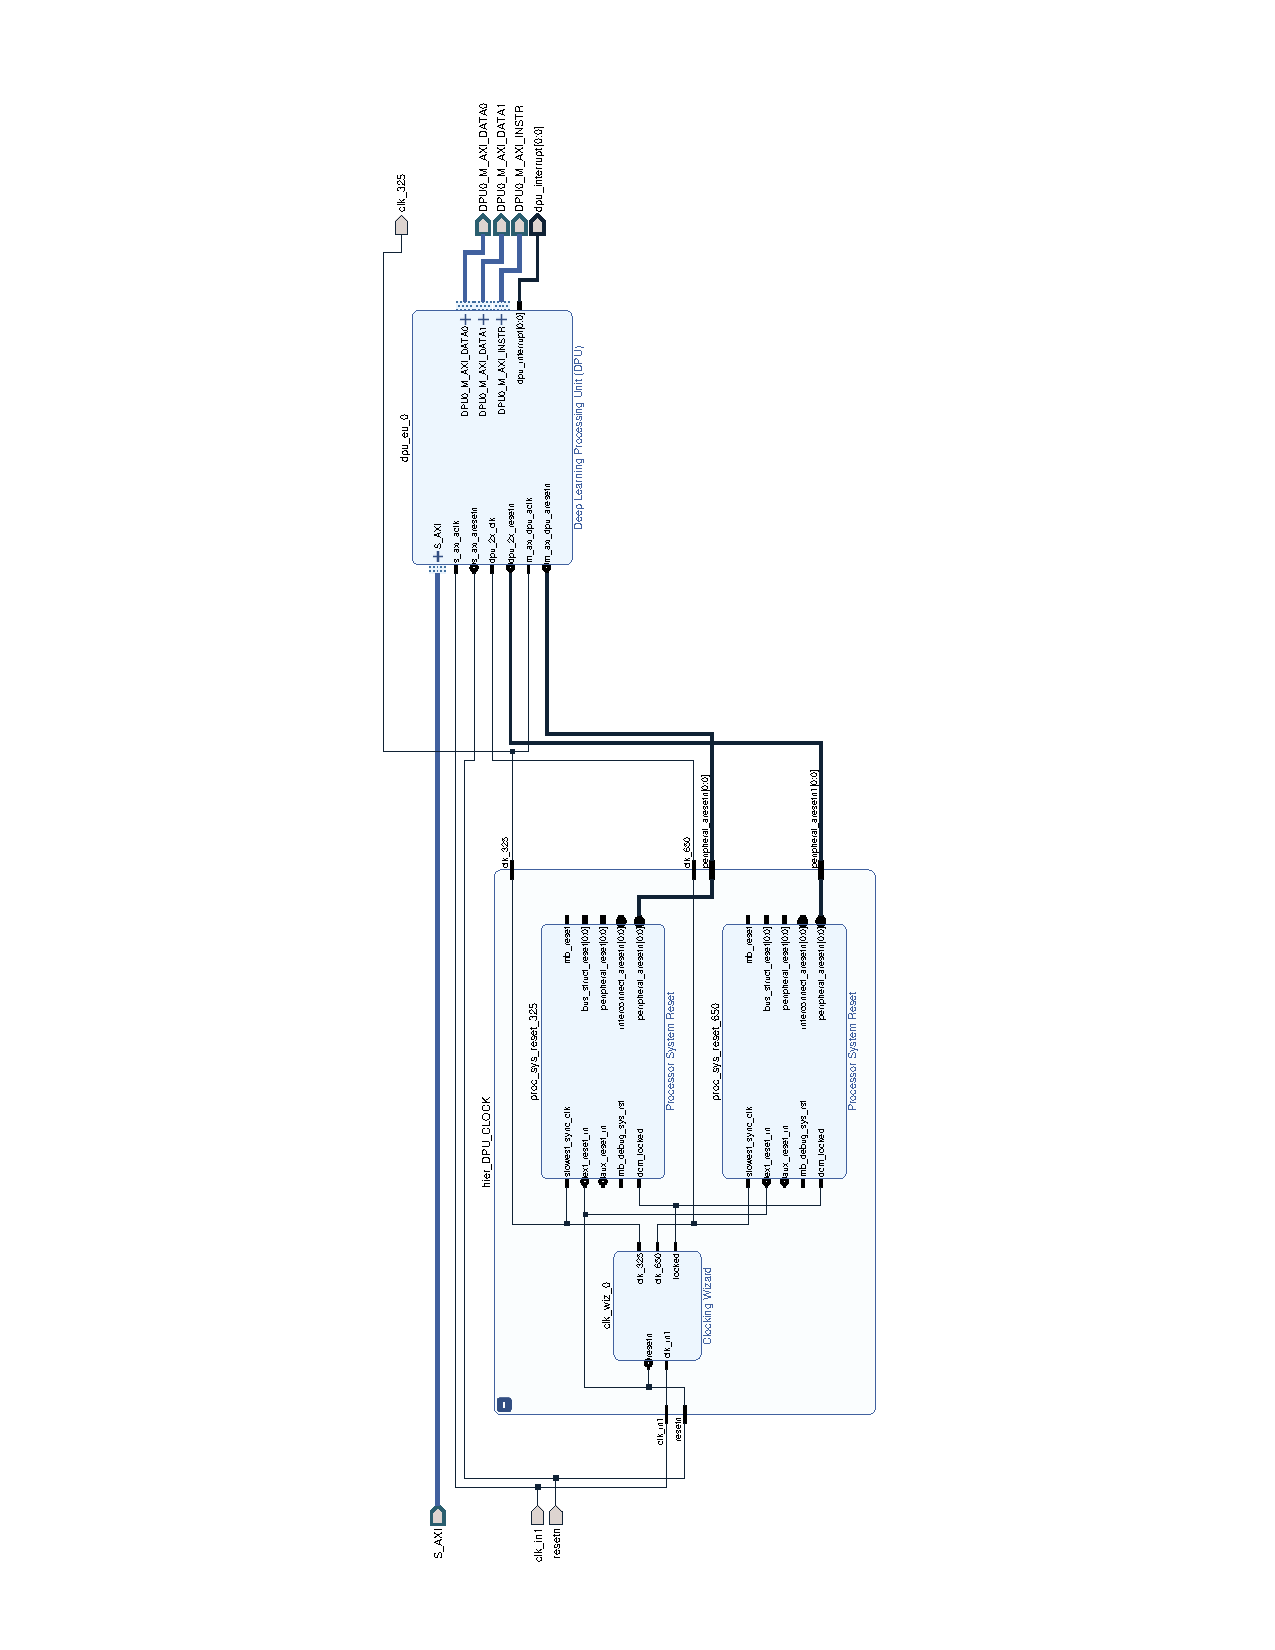
\includegraphics[width=\textwidth]{bilder/dpu_hier.pdf}
		\caption{\acs{DPU} hierarchy system}
		\label{fig:dpu_hier}
\end{figure}
Two main blocks comprise this subsystem: the clock generation and the \ac{DPU} \ac{IP} core itself. For generating the correct clock signals at appropriate frequencies a 'Clocking Wizard' \ac{IP} core is used. This block is configured to take an asynchronous reset and reference clock as input. Internally, a \ac{PLL} is used to generate faster clock frequencies which are needed for the \ac{DPU} \ac{IP} core. As this is a highly optimized hardware block, the frequency can be relatively high compared to the system block. In this design the \ac{DSP} slices are clocked with a frequency of 650 MHz. For each clock signal an asynchronous reset needs to be generated as well. This can be done via the 'Processor System Reset' \ac{IP} core. There, an asynchronous reset signal is generated for each respective clock domain. The data exchange of the \ac{DPU} \ac{IP} is handled by \ac{AXI} interfaces.
The next part of the process is building the Petalinux image files. After extracting the hardware description file and building a Linux \ac{OS} the generated system can be simulated to verify correct functionality. The tool used for this is part of the Xilinx Petalinux tool flow called \ac{QEMU}. This tool is able of emulating a Xilinx ZYNQ system in software running on a Linux host system and offers some debugging tools. After some problems trying to emulate the kernel boot operation a Xilinx employee answered my forum question regarding my particular error message. As the \ac{DNNDK} is not yet fully released, \ac{QEMU} is not able to emulate the \ac{DPU}, which is not mentioned in the documentation of either tool.
In this week on Thursday the visit to Synthara at ETH campus Irchel was scheduled and I went there with my supervisor Jelena and our marketing associate Melvin to discuss a possible collaboration in more detail. Synthara presented their rock-paper-scissors demonstrator and told us about their work flow which is quite similar to the Xilinx \ac{DNNDK}. They also presented their custom neural network used for the demonstrator, which is a very basic convolutional neural network. We agreed to developing a demonstrator together for Embedded World 2020 and made a project timetable. The work was separated among the different areas of expertise of each company with Synthara handling training the neural network and providing their custom neural network accelerator \ac{IP}. Enclustra would handle the necessary data collection and the hardware integration, both of which were my tasks.